\newpage
\subsection{Moduł mobilny lekarza}


\begin{itemize}
	\item Do modułu mobilnego, lekarz może zalogować się jedynie po stworzeniu konta w serwisie webowym. 

\vspace{0,5cm}
\begin{center}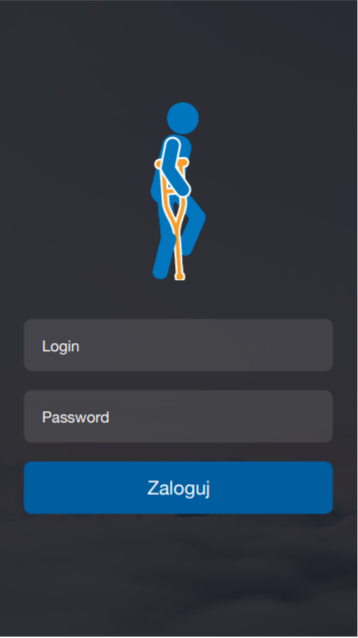
\includegraphics{obraz2/1.png}\end{center}
%\begin{center}{\scriptsize Rysunek 1: Diagram przypadków użycia.}\end{center}
\vspace{0,5cm}

\newpage
	\item Głównym ekranem, jaki widzi lekarz, jest kalendarz, z którego widzi statusy dni pracy (zielony - wszystkie terminy w danym dniu dostępne, żółty - pozostały jeszcze wolne terminy, czerwony - wszystkie terminy w danym dniu zajęte.) 
	
\vspace{0,5cm}
\begin{center}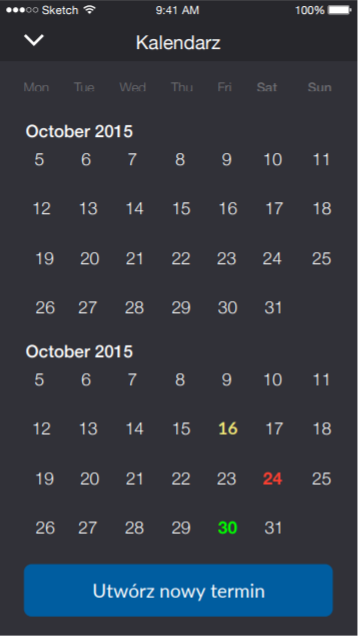
\includegraphics{obraz2/2.png}\end{center}
%\begin{center}{\scriptsize Rysunek 1: Diagram przypadków użycia.}\end{center}
\vspace{0,5cm}
\newpage
	\item Po wciśnięciu przycisku Utwórz nowy termin, otwierany jest panel, z którego można wybrać przedział czasowy trwania zabiegu, jego rodzaj oraz ustalić, czy chcemy, aby zabieg był powtarzany w poszczególnych dniach tygodnia. 
	
\vspace{0,5cm}
\begin{center}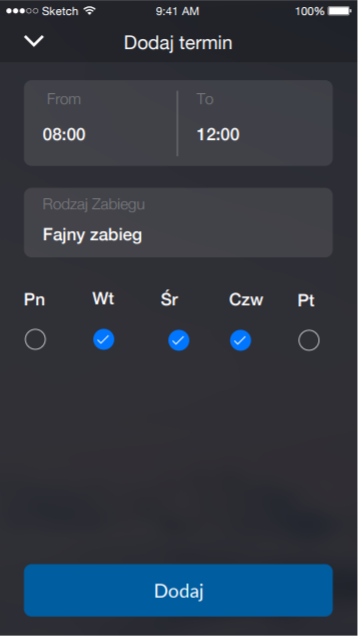
\includegraphics{obraz2/3.png}\end{center}
%\begin{center}{\scriptsize Rysunek 1: Diagram przypadków użycia.}\end{center}
\vspace{0,5cm}
\newpage
	\item Przy wyborze danego dnia z kalendarza, wyświetlany jest spis zabiegów z całego dnia, nazwa, godziny zabiegu oraz status (zajęty, potwierdzony). Z poziomu tego ekranu, możemy przesuwając przycisk z zabiegiem (w lewo - usunąć dany zabieg, w prawo - potwierdzić odbycie się zabiegu). 
	
\vspace{0,5cm}
\begin{center}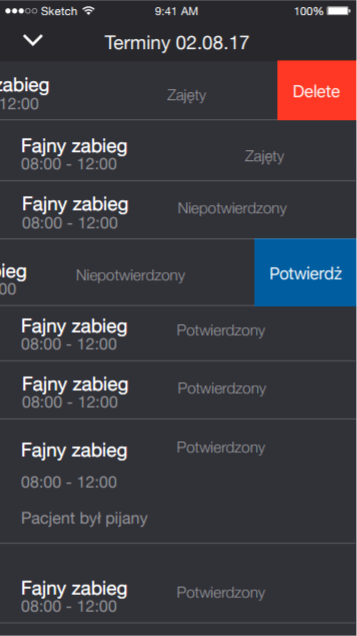
\includegraphics{obraz2/6.png}\end{center}
%\begin{center}{\scriptsize Rysunek 1: Diagram przypadków użycia.}\end{center}
\vspace{0,5cm}
\newpage
	\item Po potwierdzeniu odbycia się zabiegu, wyświetlane jest okienko, w którym możemy wprowadzić krótką notkę dotycząca przebiegu zabiegu.
	
\vspace{0,5cm}
\begin{center}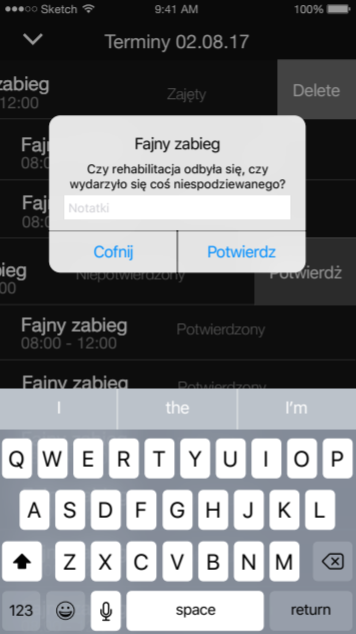
\includegraphics{obraz2/7.png}\end{center}
%\begin{center}{\scriptsize Rysunek 1: Diagram przypadków użycia.}\end{center}
\vspace{0,5cm}
\newpage
	\item Kolejną funkcjonalnością jest lista pacjentów. Z niej lekarz może wyszukać (scrollując lub używając prostego filtra po nazwisku) pacjenta. Z poziomu samej listy widoczne jest imię, nazwisko oraz email pacjenta. 
	
\vspace{0,5cm}
\begin{center}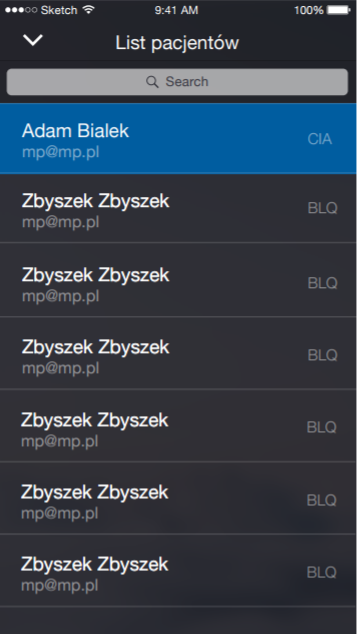
\includegraphics{obraz2/4.png}\end{center}
%\begin{center}{\scriptsize Rysunek 1: Diagram przypadków użycia.}\end{center}
\vspace{0,5cm}
\newpage
	\item Przy wyborze pacjenta z listy, widoczny jest dostęp do historii wizyt. W każdym rekordzie jest nazwa zabiegu, data przeprowadzenia, oraz opcjonalna, krótka notatka. 
	
\vspace{0,5cm}
\begin{center}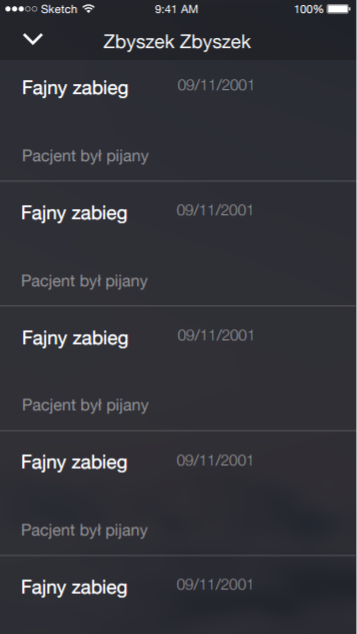
\includegraphics{obraz2/5.png}\end{center}
%\begin{center}{\scriptsize Rysunek 1: Diagram przypadków użycia.}\end{center}
\vspace{0,5cm}






\end{itemize}
